%% LyX 1.6.4.2 created this file.  For more info, see http://www.lyx.org/.
%% Do not edit unless you really know what you are doing.
\documentclass[english]{llncs}
\usepackage[T1]{fontenc}
\usepackage[latin9]{inputenc}
\usepackage{babel}

\usepackage{graphicx}
\usepackage[unicode=true, pdfusetitle,
 bookmarks=true,bookmarksnumbered=false,bookmarksopen=false,
 breaklinks=false,pdfborder={0 0 1},backref=false,colorlinks=false]
 {hyperref}

\makeatletter

%%%%%%%%%%%%%%%%%%%%%%%%%%%%%% LyX specific LaTeX commands.
%% Because html converters don't know tabularnewline
\providecommand{\tabularnewline}{\\}

\makeatother

\begin{document}

\title{Dynamic query matching}


\author{Fiona McNeill, Andriana Gkaniatsou and Alan Bundy}
\vspace{-10pt}
\institute{University of Edinburgh}
\maketitle
\begin{abstract}
This paper describes the CHAIn system, which uses data matching based on the Structure-Preserving Semantic Matching (SPSM) algorithm to match queries which are incompatible with the schema of the queried datasources to relevant parts of the schema.  These matchings are then used to rewrite the query to create relevant responses that can be returned to the original query, even though that query failed.  Despite the growing interest in intelligent query answering, we believe that this integration of data matching into query answering is unique, and allows users to successfully query datasources even if they do not know how the data in that source is organised.  We describe the process of the proof-of-concept system and briefly describe the encouraging evaluation we have so far carried out.
\end{abstract}

\section {\label{sec:Introduction}Introduction\vspace{-1mm}}
Fast, effective data sharing is essential in many situations; one of the fields in which this is particularly pressing is in the field of emergency response.  Emergency response situations are characterised by the coming together of large numbers of organisations, each of which is likely to have large amounts of data, much or some of which may be pertinent to the current emergency.  Some of these organisations may be well known to each other, but others will be unknown and potentially untrusted.  Datasources even of known organisations may be highly dynamic.  Reports into previous responses frequently cite poor communication and failure to effectively share information as a significant barrier to an effective response.  There is much interest in increasing levels of automation in this process as an attempt to address these problems \cite{pitt-report}.  There are many problems surrounding such automation; the one in which we are particularly interested is that of mismatch between data sources.

Successful querying of a datasource depends on a good understanding of that datasource, thereby ensuring that the schema of the query correctly aligns with the schema of the queried datasource.  If data querying is part of an automated process, such knowledge depends on being able to anticipate in advance exactly what datasources will be relevant and knowing accurately what the schema and data representations of that source will be at the time of querying.  In a highly dynamic environment, such as emergency response, such assumptions are often not valid.  It both precludes the possibility of dynamic interaction with new organisations not anticipated at design-time and of interacting with known organisations who have updated or altered their data in some way.  Since speed is of the essence in emergency situations, relying on human ability to identify these problems and update queries accordingly is not feasible; in addition, this depends on the ability to access the schema of other people's data, which is not always reasonable.  We therefore believe that automatic reformulation of queries based on matching between the schema of the original query and that of the queried datasource is a necessary part of automating this communication process.

This paper introduces the CHAIn (Combining Heterogeneous Agencies' INformation) system, which can be used by an owner of a datasource to formulate appropriate responses to incoming queries, even when these queries fail to match the datasource at the schema level and/or the data level.  Potential responses are ranked, and the process may be fully automated or may be used as a basis for fast, efficient human interaction with large datasources.  

The matching component of CHAIn is based on the structure-preserving semantic matching (SPSM) algorithm \cite{spsm}, originally developed in the OpenKnowledge project\footnote{http://www.openk.org/} for dynamic service integration.  The main contribution of this paper is in the adaptation of this successful matching process to the problem of dynamic query matching in (potentially) large data.

The paper is organised as follows.  Section \ref{sec:worked-ex} uses a worked example to describe the aims of the system.  Section \ref{sec:process} describes the process of the system in more detail.  Section \ref{sec:eval} discusses the results we have obtained by using this system on various emergency response datasources.  Section \ref{sec:related-work} puts our work in the context of other related work.  Section \ref{sec:concs} concludes the paper and discusses some of the key issues we need to address in developing CHAIn from a proof-of-concept system to a system that is usable in the field, and the context which is necessary to allow this.


\section{\label{sec:worked-ex}Worked Example}
We have primarily been considering this situation with relation to an emergency response scenario.  Such situations are data rich, and are characterised by the need to share data quickly and effectively with collaborators who may be previously unknown, and may not be trusted.  Formulating correct queries under these circumstances is extremely difficult, and there is therefore a pressing need for automated query reformulation.

Consider a flooding scenario.  Imagine an environmental organisation which is trying to determine how full the rivers are to anticipate the course of the floods.  They will have their own sensors monitoring this, but may want to get additional information from other organisations which also have sensors - for example, other environmental agencies from upstream regions and private companies who monitor water levels for their own commercial purposes, but may be agreeable to sharing data during an emergency.  Perhaps in their own data sources they frame readings from their sensors as follows:


%\textbf{SELECT} $reporter\_ID, node, level, date$\\
%\indent \textbf{FROM} $measurement$

$measurement(Reporter\_ID,Node,Level,Date)$

%Many organisations may require accurate, up-to-date information about where flooding has occurred
%
% have an interest in discovering where to return appropriate responses to a query on a dataset which have been (potentially) approved by an expert/owner of that dataset, together with sufficient information for the querier to determine whether or not they want to use the response.

They will then send this query to other organisations which they believe may have relevant information.  If the organisation were automatically developing queries to populate this table, the query that would be formulated would be as illustrated in Figure \ref{fig:initquery}.  If there is no mismatch at either the data or the schema level, the query will succeed and appropriate responses will be returned without the need to invoke the CHAIn system.  If, however, mismatches do occur then returning an appropriate response will require matching.  



\begin{figure}[htbp]
\begin{center}
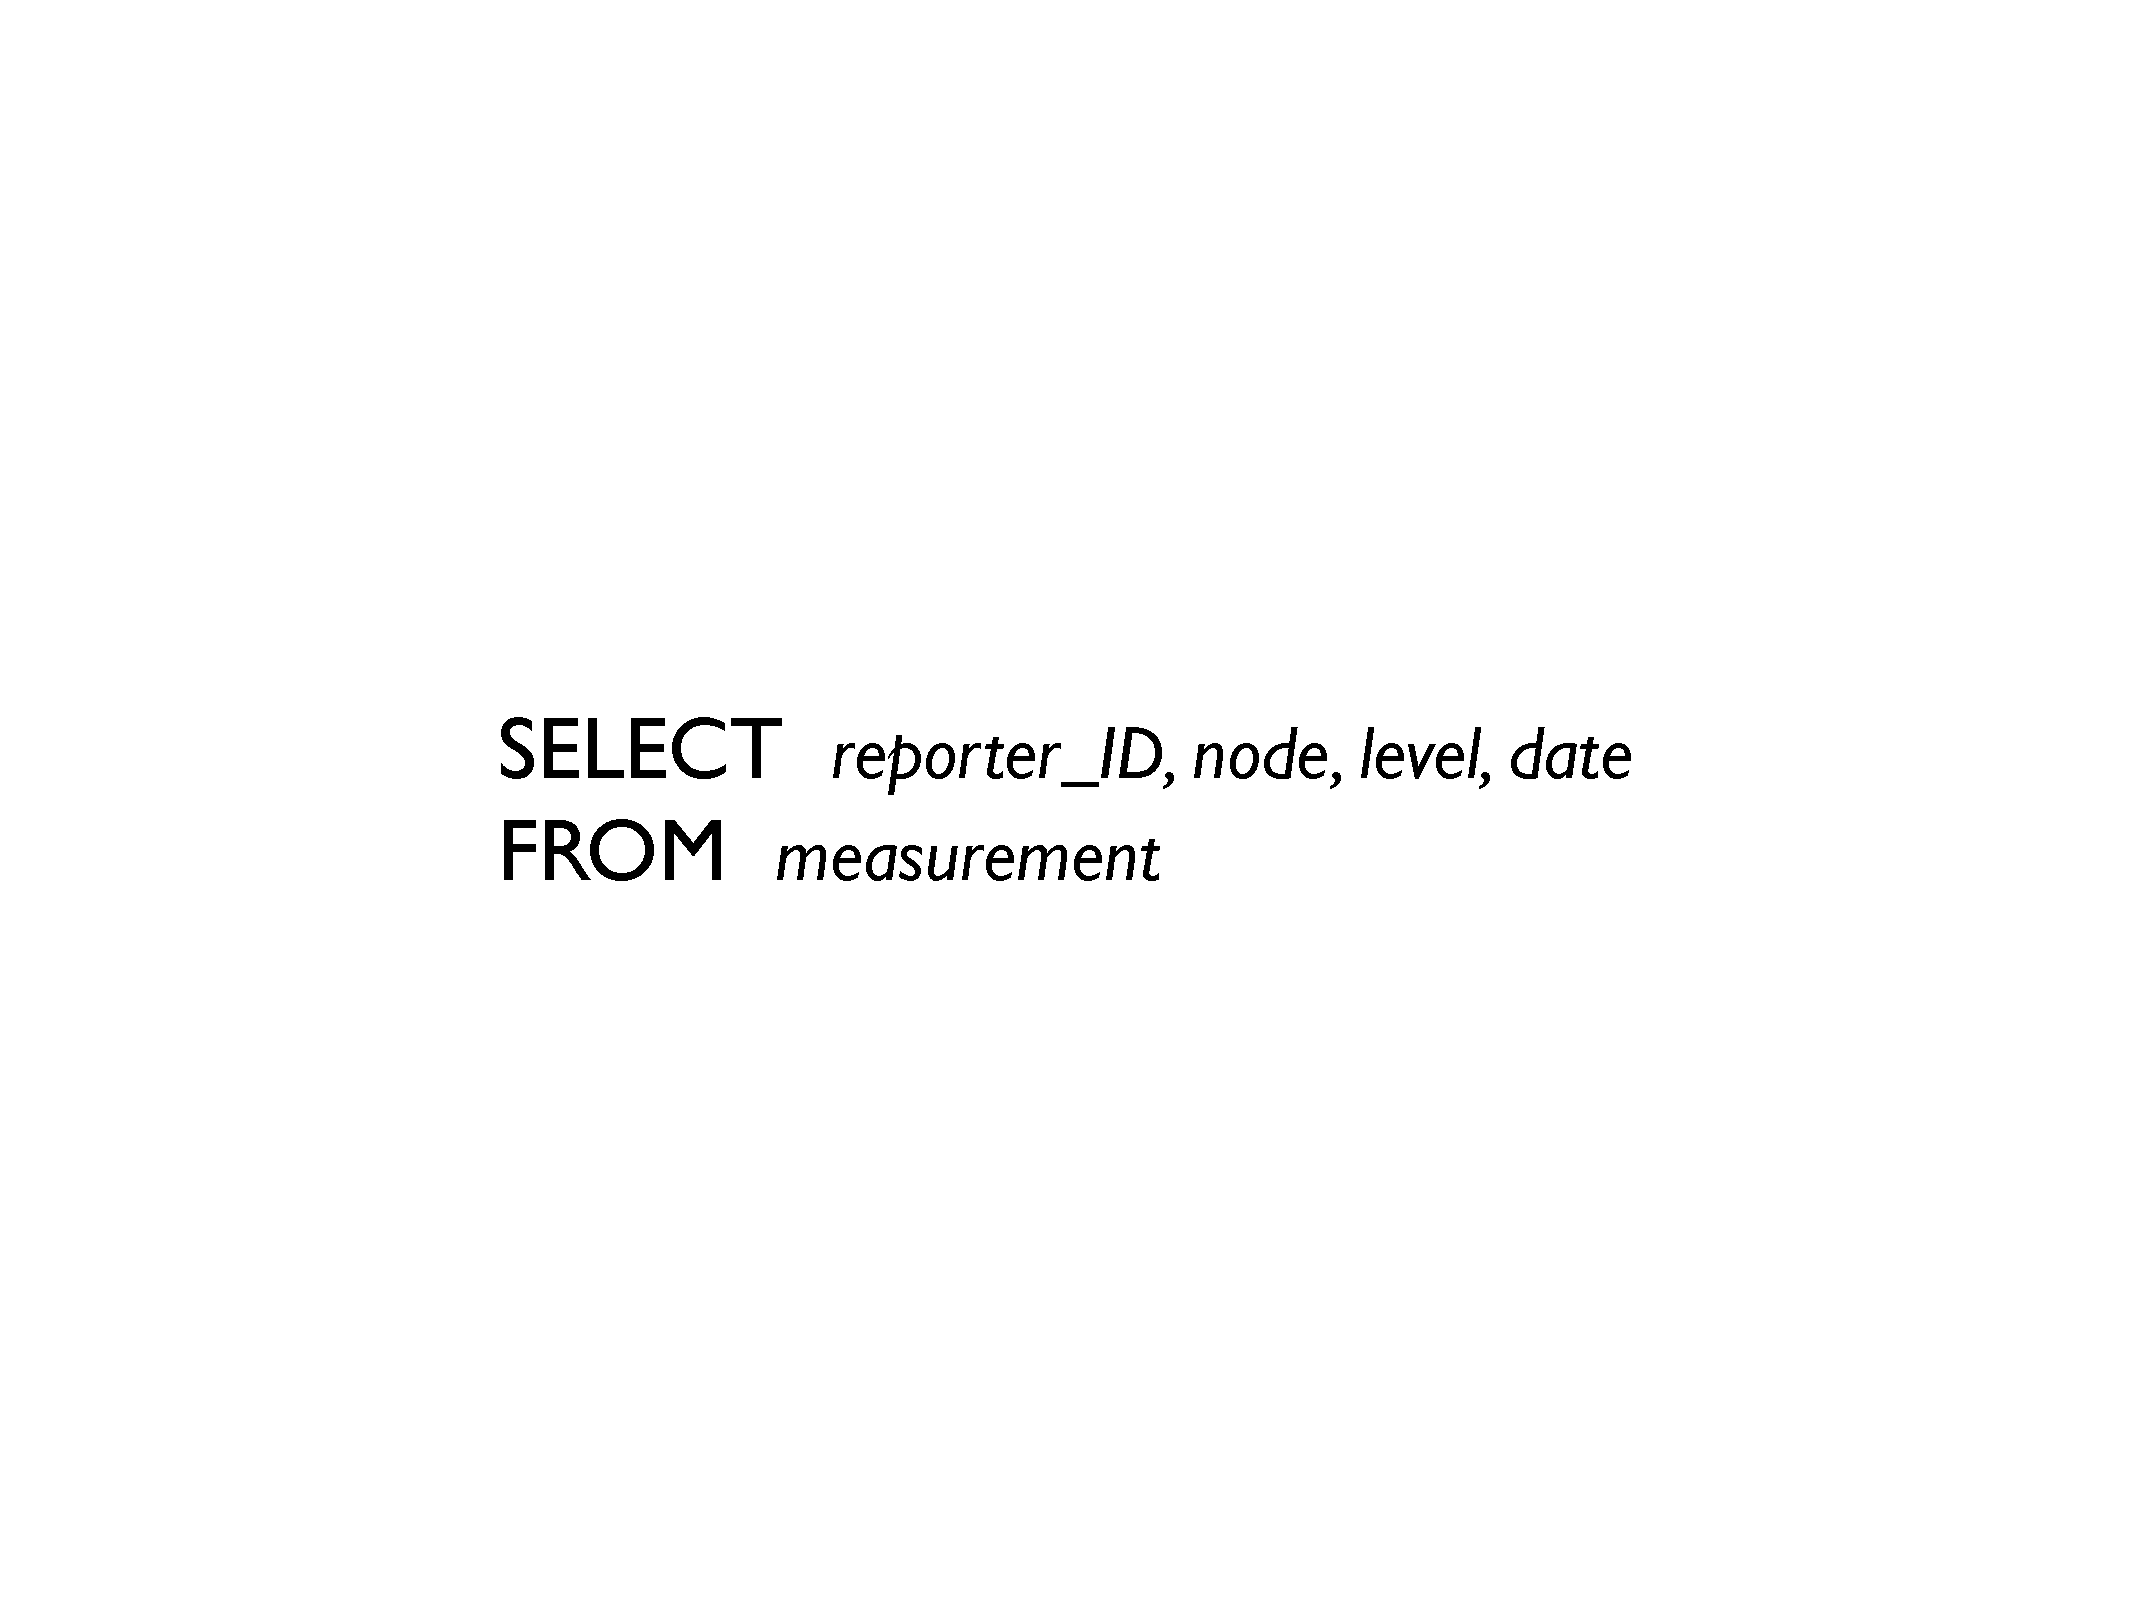
\includegraphics[width=60mm]{initquery.pdf}
\caption{Initial query based on data of querying organisation}
\label{fig:initquery}
\end{center}
\end{figure}

However, the queried organisation may organise their data differently on many levels.  Perhaps the most relevant data may be organised as follows:

$reading(Node,Date,Water\_level)$

There are various mismatches here, in the words used, in the organisation of the arguments and in the number of arguments.  The query in Figure \ref{fig:initquery} will fail.


\section{\label{sec:process}Query Response Process}
The goal of the CHAIn system is to return an appropriate response to a query on a datasource despite the fact that the query is not correctly formulated for that data source.  Whenever a query fails, CHAIn will first investigate whether the schema used by the query is correct with reference to the schema of the queried data source.  If it is not, matching is used to determine whether there is anything in the schema of the datasource which approximates to the schema of the query, and, if so, reformulates the query accordingly.  If a query fails when there is no mismatch in the schema - either because the original schema of the query was correct according to the schema of the data source, or because the query has been reformulated to reflect the schema of the datasource - the CHAIn system will then consider potential mismatches at the data level.  Ultimately, the query will be responded to using the data that CHAIn considers the most appropriate response to the original query, or it will fail if there is nothing in the queries data source which is considered sufficiently relevant.

In this section, we describe the various aspects of the process, with reference (where appropriate) to the worked example in Section \ref{sec:worked-ex}.  

\subsection{The role of humans}
CHAIn can operate completely automatically because the matching process ranks potential matches.  It is therefore possible to always choose the best match at each stage, to produce a single best-ranked response to the original query.  Setting CHAIn to be fully automated is the best approach where responses are needed very quickly and quality of matching is not important.  However, we also view CHAIn as a method for allowing human users to interact with large data sources quickly and effectively, providing them with the tools to make informed decisions.  It is therefore the general expectation that when the matching process is completed, a set of results passing a given threshold for matching quality, or constrained by the number of required results, is presented to a user that owns, or belongs to an organisation that owns, the queried data source.  These results will be presented with clear information about where approximations were made, where parts of the query were left unanswered, and so on.  This allows for the input of local knowledge into context-free matching, and helps data sources where localised terminology is used to become more universal comprehensible.  For example, $reading$ is considered by WordNet to be a direct hypernym of $measurement$, so a match may be found on that basis.  However, someone who understood the data may know that $reading$ in this context refers to book readings, and is not a correct match for $measurement$.  These kinds of poor matches are likely to be identified through poor matches in the arguments of the terms, but local input can still be valuable.

This user can decide to send back one or more (or none) of the responses suggested by CHAIn to the querier.  Again, the querying organisation can automatically accept this response if desired, or it can also be filtered by a human user within that organisation to determine whether to accept the response, or which of a list of potential responses is most appropriate.  This will depend on what the information is needed for; for example, a response missing one particular attribute of the query may be useless, whereas one missing another attribute may be of some value.  In the running example, perhaps $reporter\_ID$ is not essential because the $Node$ information can be used to determine where the reading is coming from, so a match where this is missing would be less valuable than one where it is present, but still of some use.  However, perhaps the query is primarily to discover the water level at various places, so if the attribute $water\_level$ were missing, the response would have no value to the querier.  

\subsection{Lifecycle of the Process}
\begin{enumerate}
\item A query to a particular data source is received by the organisation (or individual) that owns the data source.
\item If the query fails, it is first determined whether this is due to mismatch at the the schema level.  If not, go to step 6.  If so, naive matching is done on the schema of the datasource to narrow down the search space to likely matches (see Section \ref{sec:narrowing}).  We can assume that the schema is available without loss of privacy, because this matching is being done by a version of CHAIn which is owned by the owner of the datasource, and details of the schema need not be passed to any other party.
\item Potential matches are sent pair-wise with the query to the SPSM matcher.
\item The SPSM matcher returns matches together with a score, which can be used to reject poor matches and rank good matches (see Section \ref{sec:spsm}).
\item The query is reformulated according to the match and resent to the data source (see Section \ref{sec:reform}).
\item If the query fails, since we know at this stage that the query is correct with respect to the schema, we look for mismatches at the data level (see Section \ref{sec:reform}). 
\item Any potential responses to the query passing a given threshold are presented, with appropriate annotation describing the match, to a user who is knowledgable about the data source.  This user then choses any number of matches to be returned to the querier.  (This step can be omitted and the responses can be returned according to automatic ranking if required) (see Section \ref{sec:returning}).
\item The querier receives the response(s) to their original query, together with information about the matches that were used to produce the response, and uses these as they feel appropriate.
\end{enumerate}


\subsection{Format of the data source}
The matching part of the process matches first-order terms: that is, terms of the form $predicate(Arg_1,Arg_2, ..., Arg_N)$, where each $Arg_i$ may itself be a function.  This process is therefore applicable to data formats that can be translated into this format.  Since this is a very general format, this includes a vast number of common representations.  Currently, the CHAIn system can be used for SPARQL queries to RDF data sources and for SQL queries to RDB data sources, but it could easily be extended to be applicable to more formats.  Extending to a new format requires extensions to the querying and reformulating part of the process, but does not affect matching, the central part of the process, or the interaction with the user.

\subsection{\label{sec:narrowing}Narrowing down search space}
The matching part of the process is done by the SPSM algorithm, which does pairwise matching of structured terms.  This is an expensive process, and it is not feasible to do it between a single query and every possible match in the queried data source.  It is therefore necessary to perform a filtering step, narrowing down the (potentially large) data source to a subset of likely candidates.  This is done through fairly naive keyword matching on the predicate name of the query.  The name is annotated with synonyms, hyponyms and hypernyms, and the schema of the datasource is sorted to extract parts of it that match any of these terms\footnote{There is a considerable body of work on matching keywords, and incorporating some of this would allow us to develop a more sophisticated approach to this step of the process.  We have chosen to do this in a naive way because we are developing a proof-of-concept system, but this would be an important part of future work.}.   There is, of course, a tension in determining how wide this net should be cast: we do not wish to exclude potentially good matches; however, we do not wish to end up with a very large subset of the data, to perform complex matching on which would be very expensive.  Initial results (see Section \ref{sec:eval})  indicate our approach is workable, but extensive simulation is necessary to determine more precisely where this sweet spot lies.

After a query failure, for each of the dataset that we own, we compute the \textit{related information} given a dataset name. 	Then, given
 the dataset name of the query we try to match that name against the dataset names that we own.  Currently, this process relies 
on the SUMO and Wordnet ontologies. 
%In mored detail the steps of this process are the following:
%\begin{enumerate}
% \item Check whether a dataset name consists of multiple subwords. If so, split it into individual words.
%\item For each dataset name $D$
%    \begin{itemize}
%     \item  	Compute all SUMO related information: subClassOf, superClassOf, geographicSubRegion, overlapsSpatially
%	      \item Compute all Wordnet related information; synset, subClass, superClass, hypernym, hyponym, similar, meronym
%
%      \item For each subword $i$ $\in$ $D$:
%	    \begin{itemize}
%	      \item	Compute all SUMO related information: subClassOf, superClassOf, geographicSubRegion, overlapsSpatially
%	      \item Compute all Wordnet related information; synset, subClass, superClass, hypernym, hyponym, similar, meronym
%	    \end{itemize}
%	    


%    \end{itemize}
%\item For each SUMO and Wordnet related word:
 %\begin{itemize}
  %   \item  	Compute all SUMO related information: subClassOf, superClassOf, geographicSubRegion, overlapsSpatially
%	      \item Compute all Wordnet related information; synset, subClass, superClass, hypernym, hyponym, similar, meronym
 % \end{itemize}

%\end{enumerate}



%\subsection{Match Query Dataset Name}

%First, we check whether the dataset name provided by the query can be split into sub words. If so, we split it. To match the query dataset 
%name with the dataset names that we own we:
%\begin{enumerate}
% \item Perform string matching,
%  \item Search for possible relations.
%\end{enumerate}

%\subsubsection{String Matching}







{\bf SUMO Search}
The first step is to check whether a dataset name consists of multiple subwords\footnote{We have applied the same technique to all SUMO words, \textit{i.e. the SUMO file contains all terms that original appear in SUMO and the same terms splitted into subwords}}. 
If so, we split it into individual words. The SUMO search 
that we analyse bellow is repeated for the whole dataset name and the corresponding subwords.

\paragraph{Step 1.}\label{step1} For each non-split dataset name (single-word or mutli-word) we search for all SUMO terms that it may be related to.    
%The algorithmic steps are :

%
%\begin{itemize}
%\item For each non-split dataset name $k$ $\in$ DatasetsWeOwn,
%	\begin{itemize}
%	\item find all (non-split and split) SUMO  terms  Instance, Class, Subclass, SuperClass, SubRegion, SuperRegion, Region  such that: \\
%		\indent instance(Instance, $k$) or instance($k$, Class), and/or 
%	\\ \indent subclass(Subclass, $k$), and/or 
%		\\  \indent subclass($k$, SuperClass), and/or
%			\\	\indent  geographicSubRegion(SubRegion, $k$), and/or  
%			\\ \indent geographicSubRegion($k$, SuperRegion), and/or  
%			\\ \indent  overlapsSpattially(Region, $k$) or 	 overlapsSpattially($k$, Region).
%	
%	\end{itemize}	
%\end{itemize}
%
	

\paragraph{Step 2.} In this step we split all dataset names into lists of individual words, and for each individual word we compute all SUMO related terms.
%The algorithmic steps are :
%
%\begin{itemize}
% \item Split each dataset name $k \in DatasetsWeOwn$, into a set of subwords, such that $k=\{m_1,m_2,..,m_n\}$
%
%\item For each individual word $m_i \in \{m_1,m_2,..,m_n\}$ 
%				\begin{itemize}
%				\item find all (non-split and split) SUMO  terms  Instance, Class, Subclass, SuperClass, SubRegion, SuperRegion, Region  such that: \\
%		\indent instance(Instance, $m$) or instance($m$, Class), and/or 
%	\\ \indent subclass(Subclass, $m$), and/or 
%		\\  \indent subclass($m$, SuperClass), and/or
%			\\	\indent  geographicSubRegion(SubRegion, $m$), and/or  
%			\\ \indent geographicSubRegion($m$, SuperRegion), and/or  
%			\\ \indent  overlapsSpattially(Region, $m$) or 	 overlapsSpattially($m$, Region).
%	
%	\end{itemize}	
%\item Repeat for all $m_i \in \{m_1,m_2,..,m_n\} $
%\end{itemize} 



\paragraph{Step 3.} In this step, we split all dataset names into lists of individual words. We apply the same technique to all SUMO terms. 
Then, for each individual word that belongs to a dataset name, we search for SUMO multi-word terms which are related  that subword. 
Then, given a dataset name we compare the SUMO results and we keep only the SUMO terms that are related to more than one subwords within the same 
dataset name.
%The algorithmic steps:
%
%\begin{itemize}
%\item For each dataset $k$ where $k=\{m_1,m_2,..,m_n\}$ and $k$ $\in$ DatasetsWeOwn,
%
%\begin{itemize}
% \item Select an individual word $m_i$ $\in$ $k$,
%
%
%		\begin{itemize} 
%			\item find all SUMO split terms (lists)  Instance, Class, Subclass, SuperClass, SubRegion, SuperRegion, Region such that:\\
%						\indent instance(Instance, Class) where $m \in Instance$, or $m \in Class$, and/or\\
%						\indent subclass(Subclass, Superclass) where $m \in Subclass$ and/or $m \in Superclass$, and/or\\
%			\indent  geographicSubRegion(SubRegion, SuperRegion) where $m \in SubRegion$  and/or $m \in SuperRegion$, and/or \\
%				 \indent overlapsSpattially(RegionA, RegionB) where $m \in RegionA$ or $m \in RegionB$
%		
%\end{itemize}
%		\item repeat process for all $m_i$ $\in$ $k$
%	\end{itemize}
%\item  Keep SUMO terms which are related with more than one  individual $m_i$ $\in$ $k$,  and discard the rest.
%		 
%	\end{itemize}

  	
 {\bf Wordnet}		
In this step we only consider individual words for each dataset name. Thus, we split dataset names into lists of individual words. 
	The algorithmic steps we follow are:

\begin{itemize}
\item For each individual word $m \in k$ where $k \in QueryTerms$
			\begin{itemize}
				\item find the Wordnet id of that word
				\item  find all hyponym ids, hypernym ids, subclass ids, superclass ids , meronym ids  and similar ids which are related to $m$.
				\item for all hyponym ids, hypernym ids, subclass ids, superclass ids , meronym ids  and similar ids find the corresponding words
			\end{itemize}	
\item repeat the same process for each hyponym, hypernym, subclass,  superclass,  meronym and similar\footnote{If we are unable to split the dataset names into lists of subwords,  the above algorithms are applied in the same way, and all query terms are considered as lists with one element.}.
			

\end{itemize}
	
{\bf Schema Candidates For Matching}	
First step is to check whether the dataset name provided by the query can be decomposed to subwords. Then, we check whether the query 
dataset name, or the individual subwords, are related to the dataset names (or their subwords) of the datasets that we own. This is a two-step 
process:

\begin{itemize}
 \item[Step 1] Search suing the SUMO and Wordnet results.
\item[Step 2] Perform naive string matching.
\end{itemize}

For example, this process would find 38 related terms  predicate name $measurement$

\subsection{Structure-preserving semantic matching}\label{sec:spsm}
The Structure-Preserving Semantic Matching algorithm (SPSM) has been extensively described elsewhere (cite spsm), so we do not cover it in detail here.  Rather, we provide the reader with sufficient information to understand the principals of the process.

The SPSM algorithm requires two trees as input and returns a score in [0 1] indicating their similarity, together with mappings from each element of the source tree to elements in the target tree, or to null.  These element mappings must be $\in \{=,\subset,\supset\}$. 

SPSM is a two-step process.  We first make use of adapted conventional ontology matching techniques to investigate relationships between the individual words in the nodes of the trees. The second step matches the structure of the trees to discover an overall relationship. This is crucial because the structure of the tree itself contains a lot of semantic information that must be considered if we are determining whether two terms are equivalent or similar. SPSM, therefore, needs to preserve a set of structural properties (e.g., vertical ordering of nodes) to establish whether two trees are globally similar and, if so, how similar they are and in what way.

\subsection{Reformulating the query}\label{sec:reform}
The SPSM process will return a list of ranked responses; for example:

\noindent$1. reading(Node,Date,Water\_level)$\\
$2. measurement(Area,Wind\_speed,Direction)$

For each response, the mappings in the match are then used to reformulate the query.  Figure *?* illustrates this process.  *figure should include original  query, mappings and reformulated query*.  For aspects of the query for which mappings are found, the original term is replaced by the matched term; aspects of the query for which no mappings are found are removed from the query.  If the latter occurs, the response will not constitute a complete response to the query but may contain sufficient detail to be useful.

The repair process takes as input the mismatched query (both data and schema) and the SPSM matching results and produces new queries which are considered 
schematically correct. The repair process considers the following cases:

\begin{itemize}
 \item The query dataset name can match to more than one dataset names (which we own).
\item Each dataset match (predicate match) comes with the corresponding argument matches.
\item Within the same dataset, an argument can have more than one match (more than one arguments that can be mapped to).
\item A dataset match might correspond to more than one new query.
\item A dataset match that does not have any argument matching is discarded.
\end{itemize}

%\subsubsection*{Repair Algorithm}
%
%First step is to repair the query schema according to the SPSM results. 
%\begin{itemize}
% \item Given a query dataset name and the correspoing arguments, find all SPMS results that match the query dataset name to 
%a dataset name that we own. Keep only the dataset name matches that produce argument matches.
%\item For each $DatasetMatch_i$, where $QueryDataset \mapsto DatasetMatch_i$ find all corresponding $SingleArgumentMatches$
%    \begin{itemize}
%    \item For each $QA_i$ where $QA_i$ $\in$ QueryArguments, find all $QA_i$ that appear  one $SingleArgumentMatch$. 
%     \item Find all  $QMA_i$ $\in$ QueryArguments, that have more than one $SingleArgumentMatches$, where  $SingleArgumentMatches= \{ SingleArgumentMatch_1, \\SingleArgumentMatch_2, .., SingleArgumentMatch_n\}$ and 
%$QueryDataset(QA_i) \mapsto DatasetMatch_i(SingleArgumentMatch_1)$, \\
%$QueryDataset(QA_i) \mapsto DatasetMatch_i(SingleArgumentMatch_2)$.., and $n \leq 2$
%    \begin{itemize}
%\item  For each $QMA_i$ select randomly $SingleArgumentMatches_i$ and replace it
%
%    \begin{itemize}
%     \item Replace each $QA_i$ with the corresponding  $SingleArgumentMatch$
%      \item For each of the remaining $QA_i$ replace it with a randomly chosen  $SingleArgumentMatch_i$ 
%      \item Delete all query arguments that do not have a corresponding $SingleArgumentMatch$
%    \end{itemize}
%\item Repeat for all $SingleArgumentMatches_i$
%\end{itemize}
%
% \item Repeat untill all possible argument cobinations have been created. 
%
%
%    \end{itemize}



%\end{itemize}





%To form the final query, we have to find all data values contained in the original query and change their type. 
%Hence, for each query schema we have formed, we find (if any) the corresponding data values that are provided by the query.


\subsubsection*{Forming the final query - Data Level Repair}

The inputs of this process are all query schemata that have been formed by the previous process and for each schema the corresponding data.
For each schema we form the corresponding query and we send it to the appropriate dataset. If no answers are returned, assuming that the schema is 
correct, we  uninstantiate the data values of the query.  Goal of this process is to identify the data values that cause the query failure. 
The steps we perform are the following:

\begin{itemize}
 \item Find all data values of the query
    \begin{itemize}
    \item Select one randomly and uninstantiate it
   \item Send query to the dataset again
    \item Check if it returned any answers
	\begin{itemize}
	
	\item If no answers were returned, pick another data value, and uninstantiate it 
	  \item Send the new query to the dataset
	  \item Check for answers
	\end{itemize}
      \item Repeat for all data values
      \end{itemize}

    \item Uninstantiate all data values of the query
    \item Send uninstantiated query to the appropriate dataset
      
\end{itemize}

The system currently does no matching at the data level, instead returning all responses which match some of the query data, or, if necessary, only the schema of the query. It is obviously possible to include matching at the data level to produce more appropriate responses, and this is something we intend to do in the future.

%{\bf Data-level matching}
%The reformulated query is then submitted to the datasource.  If failure now occurs, this cannot be to do with schema mismatch because the reformulated query must be correct according to the schema of the datasource.  We can therefore conclude that the query failed because no matches were found at the data level.  This may be because the datasource simply does not contain pertinent information; however, it may be because mismatches at the data level led to potentially relevant data not being recognised.  We therefore continue matching at the data level to determine whether a suitable response to the original query can be extracted from the data source, or whether failure of the query is in fact the appropriate response.
%
%*more detail about how this is performed*.
%

\subsection{Returning query responses}\label{sec:returning}
Up to this point, the process has been fully automated and, as mentioned earlier, it is possible to run the CHAIn system without any user interaction if desired.  However, we feel\footnote{more extensive evaluation is necessary to clearly demonstrate this} that some level of user interaction will be important in improving the quality of results.  We also see the CHAIn system as a useful tool in allowing efficient human interaction with large datasource, guiding the human as to how to appropriately respond to queries to the datasource by reducing a large datasource to a handful of potential responses, together with information to help them understand in what way the responses answer the query, and which aspects of the query are unanswered.

Helping users, who may have a good understanding of the data used by their organisation, but are unlikely to be experts in representation and matching, to appropriately and efficiently evaluate a set of potential responses to a query, weighing them against each other with reference to the particular ways in which each individual response fails to be an exact response to the original query, is a complex and demanding task, requiring high-quality techniques in human-computer interaction.  Whilst building such expertise into the system will be essential before this approach is usable in the field, we do not pretend to such expertise ourselves, and therefore have a much simpler approach to user interaction, with a complete approach to this relegated to future work.


\section{\label{sec:eval}Evaluation}
Large-scale evaluation of this kind of matching is difficult.  This is chiefly because:
\begin{itemize}
\item we need to develop specific queries in each case, ideally generated from data and schema from existing datasources;
\item these need to be sent to a datasource from which we could realistically expect an answer - that is, the query and the receiving datasource need to be similar enough to expect results;
\item we need to analyse the results, with the help of experts where appropriate, to judge whether or not the responses are appropriate;
\item we need to examine the receiving datasource to see if there were any appropriate responses which were not returned.
\end{itemize}
A robust evaluation of this approach requires these queries to be generated during the kind of automated process we envisage this work be used in, and the effective of these matches determined through large-scale simulation, to determine what the actual impact of using these matches are.  This is outside the scale of our current project (see Section \ref{sec:concs} for discussions of our plans to do this).

We have therefore carried out the evaluation as follows:
\begin{enumerate}
\item We have sourced appropriate data from a collaborator, SEPA (Scottish Environmental Protection Agency).
\item We have sourced online various different datasource which discuss similar things, such that we might expect a query from such a datasource to have some chance of finding an appropriate response in our SEPA data.
\end{enumerate}

We have so far carried out 26 evaluation tests.  Of these, 14 returned responses to the queries, which in all cases were judged appropriate.  12 did not return a result.  In 4 of these cases, this was because the narrow-down process returned no results, and in all cases this was judged an appropriate response because there was nothing in the target datasources which matched the query predicate name (not returning irrelevant results is almost as important as returning relevant results).  8 of these failed at the SPSM matching after receiving input from the narrow-down process.  Of these, 3 were appropriate failures, because the arguments of the narrowed-down predicates were not similar enough to the query to justify return data; 5 failed because of implementational issues which we believe can be fixed without difficulty.

In this section, we present two tests, to give a flavour for the results we have achieved.  In all both cases the data is mapped to SEPA datasets.

\indent freshWaterResources( resource, measure, geo, timePeriod)
\subsection{Test 1}

\indent \texttt{ water( resource, measure, geo, timePeriod)}, based on data from the European Fresh Water Resources dataset

\paragraph{Plural: On, Results: *what does this mean?* } The narrow-down process returned the following possible candidates:

\begin{itemize}
\item waterBodyPressures
\item waterBodyMeasures
\item surfaceWaterBodies
\item bathingWaterLocations

\end{itemize}

The results we obtained from SPSM are the following: 


\textbf{Match 1.}\\
 water $\mapsto$ waterBodyPressures \\
water(timePeriod) $\mapsto$ waterBodyPressures(identifiedDate)\\
water(geo) $\mapsto$ waterBodyPressures(waterBodyId)\\
water(measure) $\mapsto$ waterBodyPressures(assessmentCategory)\\
water(resource) $\mapsto$ waterBodyPressures(source)\\





\subsubsection{Test 2} 

This query is formed from the UK Environmental Agency Bathing Waters dataset schema:
\indent \begin{small}\texttt{ uk$\_$BathingWaters( sampleClassification, prefLabel, long, lat, northing, easting,  latestComplianceAssessment, type, country, district,  envelope, latestBathingWaterProfile, sedimentTypesPresent, uriSet, regionalOrganization, yearDesignated, latestSampleAssessment, eubWidNotation, waterQualityImpactedByHeavyRain, zoneOfInfluence, samplingPoint, complianceClassification, primaryTopic, extendedMetadataVersion, definition, label)}\end{small}

\paragraph{Plural: On, Results: } The narrow-down process returned the following matching candidates: 

\begin{itemize}
\item  bathingWaters
\item bathingWaterLocations
\item waterBodyMeasures
\item waterBodyPressures
\end{itemize}
SPSM retuned the following matches: 

\textbf{Match 1.}\\
uk$\_$BathingWaters $\mapsto$ waterBodyMeasures\\
uk$\_$BathingWaters(label)$\mapsto$ waterBodyMeasures(waterBodyId)\\
uk$\_$BathingWaters(primaryTopic)$\mapsto$ waterBodyMeasures(secondaryMeasure).

\textbf{Match 2.}\\
uk$\_$BathingWaters $\mapsto$ waterBodyPressures\\
uk$\_$BathingWaters(label)$\mapsto$  waterBodyPressures(waterBodyId)\\
uk$\_$BathingWaters(type) $\mapsto$ waterBodyPressures(pressureType)\\
uk$\_$BathingWaters(prefLabel) $\mapsto$ waterBodyPressures(activity)\\
uk$\_$BathingWaters(sampleClassification) $\mapsto$  waterBodyPressures(affectsGroundwater)

\textbf{Match 3.}\\
uk$\_$BathingWaters $\mapsto$ bathingWaters.\\
uk$\_$BathingWaters(label) $\mapsto$ bathingWaters(description)\\




\section{\label{sec:related-work}Related Work}
The work in this paper is concerned with applying techniques that have already been evaluated and used in other contexts to a new domain.  The SPSM algorithm is novel in that whilst it is built on standard tree-edit-distance techniques (e.g., in (cite tree matching), using semantic matching to determine what impact on the overall meaning of a tree altering or removing will have.  Previously, it has been used to perform service integration and peer selection in a peer-to-peer network \cite{trust}.  The novelty of our work is in developing a system that can use this structured matching techniques to address the problem of returning useful results to a query on a datasource which has not been correctly formulated according to the schema and data within that datasource.

There is a considerable body of work (*is there?*) on the problem of intelligent query answering, which aims to do more than simple look-up based on the query.  However, this work tends to focus on different problems than the one we are interested in.  The issue generally addressed concerns how to return maximum, or maximally useful information and may use information within the datasource - for example, a concept hierarchy - to return information relevant to terms not directly included in the query.  However, it is not generally concerned with the problem of querying a datasource with which one is not familiar, so that the terms and structure used may be wholly or partially inappropriate for the datasource: the need to use matching techniques is not considered.

(cite Han et al) describes various approaches to this issue, where intelligent query answering is used to provide more (relevant) detail  than the query originally asked for, to provide summaries of data, and to rewrite queries into sub-queries.  However, the issue of data matching is not considered; rather, the question is about how much relevant information can be returned, assuming the query is correctly formed.  Work looking into intelligent query answering tend to assume far more complex databases than we have considered, where deduction rules, concept hierarchies and knowledge discovery tools are available.  We have kept our attention focussed on simple databases because we believe these are most common in the emergency-response scenario we are focussing on; however, investigating the combination of our matching techniques with intelligent-query-answering techniques for situations where more complex databases were available would be very interesting and could result in a more sophisticated approach to query answering.  (cite Han et al) also raises interesting questions about how to appropriately interact with the user and how to ensure that sensitive data is released in an appropriate way to appropriate people, which are also very relevant to an in-the-field version of our work.  *Also brief sentence about the other intelligent query answering paper*

Work has also been done on combining data from different sources to provide intelligent responses to queries (see, for example (cite hagedorn paper), but the problem of data mismatch is not considered.  *Sentence about semantic similarity in Buscaldi and Hollink papers)


\section{\label{sec:concs} Conclusions and Further Work}
The problem of successfully querying unknown datasources is an important one in terms of developing the vision of the Semantic Web, where interactions can be dynamic and unpredictable.  The general assumption in database querying is that the querier knows the datasource and can use the correct schema and terminology when developing their query, but this is a massively limiting assumption as it restricts querying to situations where: 1) one knows in advance what datasources one will wish to query; 2) one has the time to devote to examining the datasource and correctly formulating any queries one may have; 3) the datasource is open and one can examine its schema.  We believe this discounts a large number of situations in which one or more of these assumptions are not valid, and we particularly motivate this with reference to an emergency response situation, where collaborations are formed dynamically and quickly, where information needs to be passed rapidly, and where the size, number and potential sensitivity of available datasources ensure that it is impossible to adequately understand all relevant data.

The CHAIn system described in this paper uses an established structural matching algorithm - SPSM - to address the problem of mismatched database queries.  We are centrally interested in how techniques developed for ontology matching can be used to address other situations in which data mismatch of some sort is a problem.  CHAIn is currently a proof-of-concept system and requires significant further development and extensive evaluation based on simulation before we expect it to be usable in the field.  However, the implementation and evaluation we have produced so far have demonstrated that this approach to queries which are mismatched with the datasource they are querying is valid and potentially useful.

There are many ways in which we intend to extend this work.
\begin{itemize}
\item Extending the matching techniques, for example to be more domain-sensitive and to include matching at the data level.
\item Building in information about provenance and trust so that users of the system have more confidence in query responses.
\item Developing more sophisticated ways to interact with users.
\item Integrating the matching system into a larger system which controls the interactions during emergency responses (e.g., how organisations identify and interact with one another).
\item Extending the system to cope with more sophisticated datasources, and integrating techniques from intelligent query answering.
\item Extensive evaluation based on simulation.
\end{itemize}




\bibliographystyle{plain}
\bibliography{bibfile}




%Frege, G. (1892) "On Sense and Reference", in Ludlow, P. (ed.) (1997) Readings in the Philosophy of Language, Cambridge, Mass.: MIT, pp. 563-583.

%Vander Wal, T. (2005) "Explaining and showing broad and narrow folksonomies", online at http://www.vanderwal.net/random/entrysel.php?blog=1635




\end{document}
